\documentclass[a4paper]{article}
\newcommand\hmmax{0}
\newcommand\bmmax{0}
\usepackage{booktabs}

%% Language and font encodings
\usepackage[english]{babel}
\usepackage[utf8x]{inputenc}
\usepackage[T1]{fontenc}
\usepackage{gensymb}
\usepackage{pdfpages}
\usepackage{enumitem}
\usepackage{mathtools}
\usepackage{natbib}
\setcitestyle{authoryear}
\bibliographystyle{unsrtnat}

%% Sets page size and margins
\usepackage[a4paper,marginparwidth=1cm, left=1cm, right=1cm, top=2.54cm, bottom=2.54cm]{geometry}
\usepackage[toc,page]{appendix}

%% Useful packages
\usepackage{amsmath}
\usepackage{bm}
\usepackage{listings}
\usepackage{multirow}
\usepackage{array}
\usepackage{amssymb}
\usepackage{float}
\usepackage{graphicx}
\usepackage[colorinlistoftodos]{todonotes}
\usepackage[colorlinks=true, allcolors=blue]{hyperref}
\usepackage[final]{matlab-prettifier}
\usepackage{courier}
\usepackage{algorithm}
\usepackage[noend]{algpseudocode}
\usepackage[]{appendix}
\usepackage[final]{matlab-prettifier}
\newcommand*{\vertbar}{\rule[-1ex]{0.5pt}{2.5ex}}


\usepackage[bitstream-charter]{mathdesign}
\let\circledS\undefined
\usepackage[T1]{fontenc}
\DeclareMathAlphabet{\altmathcal}{OMS}{cmsy}{m}{n}
\setlist[itemize]{noitemsep, topsep=2pt}
\setlist[enumerate]{noitemsep, topsep=2pt}

\title{\vspace{-3cm}AIMS CDT: Online Learning and Multi-Armed Bandits}
\author{Mrinank Sharma}
\date{}

\begin{document}
	\maketitle
	
	\section{Introduction}
	In the Multi-Armed Bandit (MAB) problem, an agent (or algorithm) is required make decisions under uncertainty over a number of sequential steps in order to maximise a reward function, or equivalently, to minimise a loss function. This type of problem is found often in the real-world, including the ad selection problem, where an algorithm must determine which ad to display to a user, as well as in medical trials, where a doctor must decide which treatment to provide a patient.
	
	Here, we focus on stochastic bandits for which the rewards provided by each arm are drawn according to some underlying distribution for each arm. We consider different algorithms to solve this problem, and empirically compare them their performance in terms of \emph{regret}. 
	
	\section{Preliminaries}
	\subsection{Problem Definition}
	The algorithm chooses between $K$ different actions (also refered to as arms) across $T$ rounds. For the stochastic bandit problem, rewards provided by arm $a \in  \lbrace 1, \ldots, K \rbrace$ are drawn according to some fixed (but unknown) distribution, $\altmathcal{D}_a$. Denote the chosen action at round $t$ as $a_t$. Then, the reward at this timestep, $r_t$, is
	\begin{align}
	\text{Pr}(r_t | a_t = a) = \altmathcal{D}_a(r_t).
	\end{align}
	The regret at round $T$ is defined as:
	\begin{align}
	R(T) \triangleq \mu^* \cdot T - \sum_{t=1}^{T} \mu(a_t)
	\end{align}
	where
	\begin{align}
	\mu(a_t) = \mathbb{E}_{r \sim D_{a_t}}[r_t],
	\end{align}
	and $\mu^* = \max_{a} \mu(a)$. The maximiser of this will be denoted as $a^*$. The regret compares the performance of the algorithm with playing the best possible action ($a^*$) at each round. 
	
	Many of the algorithms that we will consider will require a notion of a \emph{confidence radius}, representing a region around the empirical means which we believe that the true mean will lie in. Typically, the confidence radius is chosen to be of the form:
	\begin{align}
	r(a) = \sqrt{\frac{2 \log T}{n_a}}
	\end{align} 
	where $n_a$ is the number of times which arm $a$ has been played. This choice is made so that:
	\begin{align}
	Pr[|\overline{r_a} - \mu_a| > r(a)] \leq \frac{2}{T^4}
	\end{align}
	where $\overline{r_a}$ is the sample mean of the rewards provided by arm $a$. Intuitvely, we require that the probability of the sample mean being far from the true mean (which we will refer to as the `bad event') decays quickly enough, and this motivates this choice. Note that the above bound is typically derived using Hoeffding's inequality, which only applies for bounded random variables. 
	
	Here, we will consider the following algorithms: (1) Explore-first (2) Upper Confidence Bound (UCB) (3) $\epsilon$-Greedy (4) Thompson Sampling. Note that this is an (approximate) Bayesian approach, which requires the definition of priors over arm parameters. We will also focus on the cases where $\altmathcal{D}_a$ are Bernoulli or Gaussian random variables. Please see \cite{book} for an overview of these algorithms. 
	
	\subsection{Confidence Radius for Gaussian RVs}
	The proof that the probability of a bad event decays with $T^4$ does not hold for Gaussian random variables, because these random variables have infinite support. However, we now prove a similar tail bound for these variables and thus derive a confidence radius. 
	
	Let $r_a \sim \altmathcal{N}(\mu_a, \sigma^2)$, and suppose that $\lbrace r_a^{(1)}, \ldots, r_a^{(n_a)} \rbrace$ are samples from this distribution. We need to consider:
	\begin{align}
	\text{Pr}\Big[ \Big| \underbrace{\frac{1}{n_a} \sum_{i=1}^{n_a} r_a^{(i)} - \mu_a}_{Z} \Big| > t \Big].
	\end{align}
	Using the properties of Gaussian RVs, $Z \sim \altmathcal{N}(0, \sigma^2 / n_a)$. Then, 
	
	\begin{align}
	\text{Pr}[|Z| > t] &= 2\ \text{Pr}[Z > t] \tag*{(Symmetry)} \\
	&= 2\ \text{Pr}[\exp(\lambda Z) > \exp(\lambda t)] \tag*{(For $\lambda > 0$)} \\
	&\leq \frac{2\  \overbrace{\mathbb{E}[\exp(\lambda Z)]}^{\text{MFG}_Z(\lambda)}}{\exp(\lambda t)} \tag*{(Markov's Inequality)} \\
	&= 2\ \exp(\frac{\sigma^2 \lambda^2}{2 n_a} - \lambda t),
	\end{align}
	By subsituting the closed form expression for the Moment Generating Function (MGF) for Gaussian RVs. Then, minimising the upper bound over lambda yields:
	\begin{align}
	\text{Pr}[|Z| > t] \leq 2 \exp(\frac{-n}{2\sigma^2} t^2).
	\end{align}
	Thus, setting
	\begin{align}
	r_a(t) = \sqrt{\frac{8 \sigma^2}{n} \log T}, \label{gaussian_rad}
	\end{align}
	gives the probability of the bad event decaying with $T^4$, even though Gaussian RVs have infinite support. It is pleasing that this equation scales linearly with $\sigma$, as we expect that larger $\sigma$ should give a larger confidence radius. 
	
	\subsection{Thompson Sampling for Gaussian RVs}
	In order to implement Thompson Sampling, we need to be able to compute the posterior on arm parameters. We will use conjugate prior distributions, thus using a Beta and Gaussian prior for the Bernoulli and Gaussian arms respectively. The update equations for the Bernoulli arm posterior is found in \cite{thompson}, so all that remains is to derive the update equations for Gaussian arms.
	
	Consider arm $a$. The rewards from this arm have a Gaussian distribution i.e., 
	\begin{align}
	r_a \sim \altmathcal{N}(\mu_a, \sigma_a^2).
	\end{align} 
	We will consider $\sigma_a^2$ to be a known parameter, whilst $\mu_a$ is unknown. We place a Gaussian prior on the mean:
	\begin{align}
	p(\mu_a) = \altmathcal{N}(\mu_a | \hat{\mu}, \hat{\sigma}^2).
	\end{align}
	The posterior will be updated in a sequential way (i.e. using \emph{online learning}). Suppose that $\lbrace r_a^{(1)}, \ldots, r_a^{(n_a)} \rbrace$ are samples from this arm. Then, by Bayes' rule:
	\begin{align}
	p(\mu_a | r_a^{(1)}, \ldots, r_a^{(n_a)}) \propto \underbrace{p(\mu | r_a^{(1)}, \ldots, r_a^{(n_a - 1)})}_{``\text{prior}"}  \underbrace{p( r_a^{(n_a)} | \mu_a)}_{\text{likelihood}},
	\end{align}
	where the first term is effectively acting as a prior. Suppose that this effective prior is Gaussian with mean $\mu_p$ and variance $\sigma_p^2$. Then, the posterior is also Gaussian with the following form. 
	\begin{align}
	p(\mu_a | r_a^{(1)}, \ldots, r_a^{(n_a)}) = \altmathcal{N} \Big( \mu \Big|\ \frac{\mu_p \sigma_a^2 + r_a^{(n_a)} \sigma_p^2 }{\sigma_a^2 + \sigma_p^2}, \frac{\sigma_p^2 \sigma_a^2}{\sigma_a^2 + \sigma_p^2} \Big)
	\end{align}
	The above equation provides a way to update the posterior on $\mu_a$ as additional observations of the reward arrive. Then, the normal Thompson sampling approach can be applied. 
	
	\section{Simulations}
	\subsection{Bernoulli Arms}
	We draw $K=5$ Bernoulli arms, sampling the mean parameter according to $\text{Beta}(1, 1)$. This is then set to be the prior distribution on the mean of each Bernoulli distribution. We implement the explore-first algorithm setting $N = T^{2/3} (\log T)^{1/3}$, where $N$ is the number of times each arm is explored before the exploit stage of the algorithm. This is the setting used to derive regret bounds in \cite{book}. Additionally,  we use $\epsilon = t^{-1/3} (K \log t)^{1/3}$ for the $\epsilon$-greedy algorithm, which is again the value used to derive regret bounds. 
	\begin{figure}[H]
		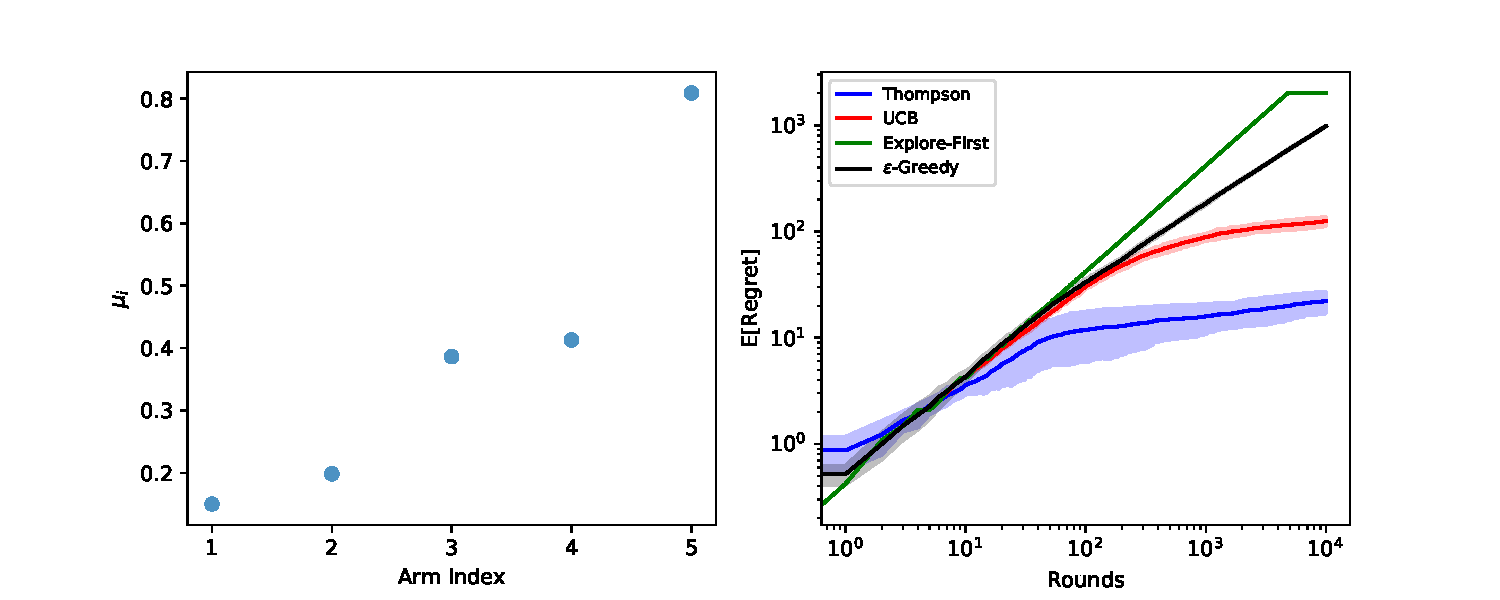
\includegraphics[width=\textwidth]{bernoulli}
		\centering
		\caption{\label{bernoulli}Simulation results using Bernoulli arms. Left: distribution of mean values of each arm. Right: expected cumulative regret for the different algorithms considered here. }
	\end{figure}

	\subsection{Gaussian Arms}
	We draw $K=10$ Gaussian arms, sampling the mean parameter according to $\altmathcal{N}(0.5, 1)$. The variance of the each arm is set to be $\sigma^2 = 0.1^2$, and this is the same across all arms. We consider setting the prior distribution on the mean value of each arm to be the ``correct" prior (i.e. the distribution according to which the mean was sampled) as well as $\altmathcal{N}(1, 0.25^2)$ (labelled ``A") and $\altmathcal{N}(-1, 0.25^2)$ (labelled ``B").  We use the same configurations for parameters of the explore-first algorithm and $\epsilon$-grredy algorithm as for the Bernoulli arms, but we use Eq.~\eqref{gaussian_rad} as the confidence range for the UCB algorithm. 
	\begin{figure}[H]
		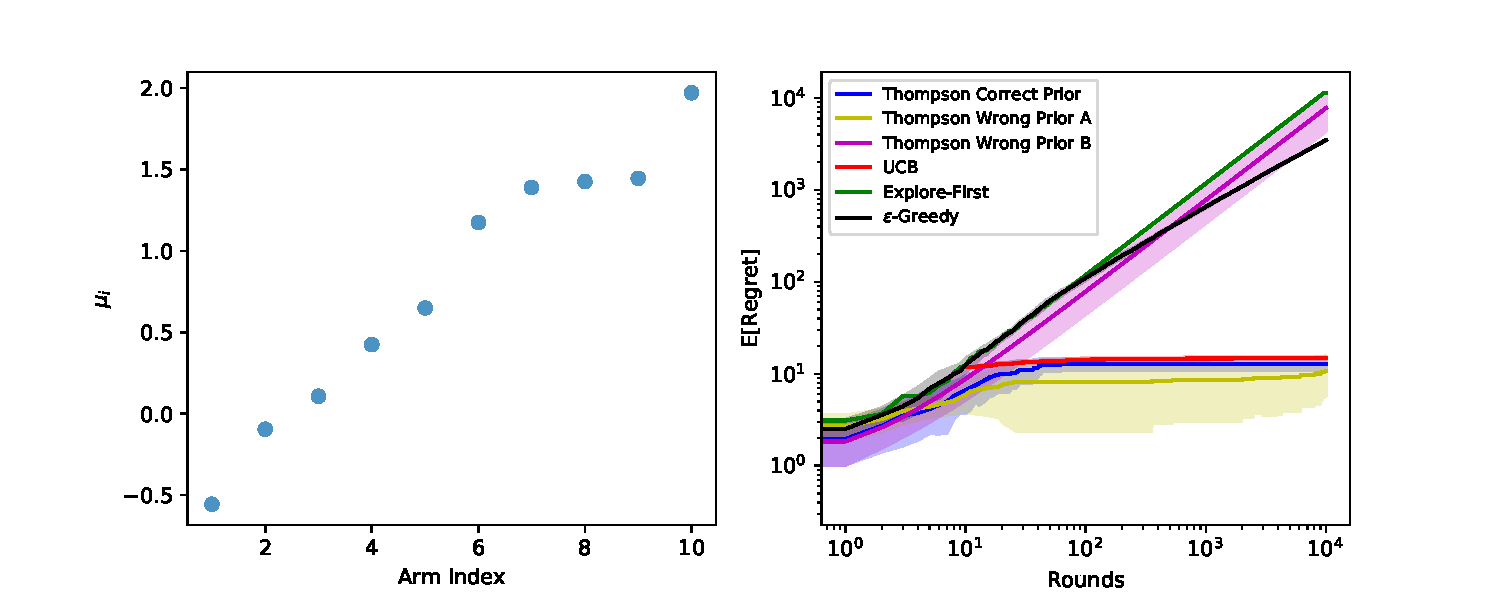
\includegraphics[width=\textwidth]{gaussian}
		\centering
		\caption{\label{gaussian} Simulation results using Gaussiani arms. Left: distribution of mean values of each arm. Right: expected cumulative regret for the different algorithms considered here.}
	\end{figure}
	\section{Conclusions}

\bibliography{sample}

\end{document}